\documentclass{article}
\usepackage[utf8]{inputenc}
\usepackage{amsmath}
\usepackage{amsfonts}
\usepackage{graphicx}
\usepackage{float}

\title{Análisis Exploratoio de Longley}
\author{}
\date{}

\begin{document}

\maketitle

\begin{itemize}
    \item \textbf{GNP.deflator (Gross National Product Deflator)}
    \begin{itemize}
        \item \textbf{Descripción:} Índice del nivel de precios de la economía, que refleja la inflación.
        \item \textbf{Escala:} Cuantitativa Continua.
        \item \textbf{Significado:} Mide el nivel general de precios relativos a un año base y cómo han cambiado con respecto a ese año. Representa la relación entre el producto nacional bruto (PNB) nominal y real.
    \end{itemize}
    \begin{figure}[H]
        \centering
        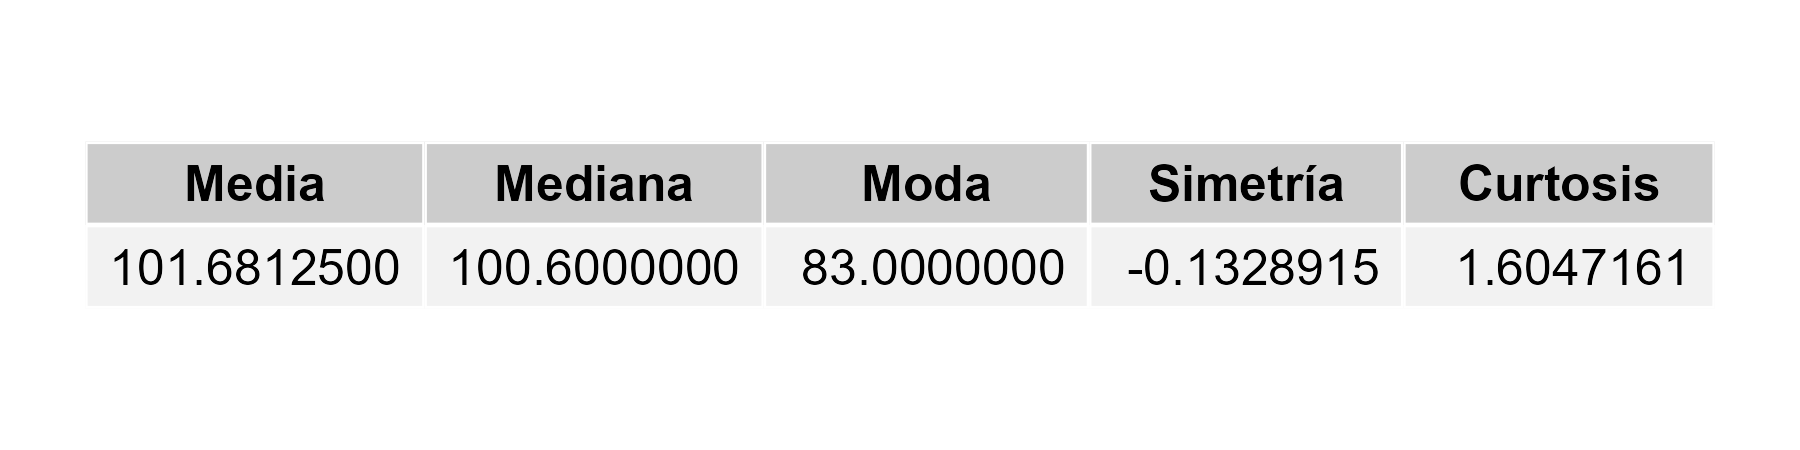
\includegraphics[width=\textwidth]{MTC/GNP.deflator_central.png}
        \caption{Medidas de Tendencia Central para GNP.deflator}
    \end{figure}
    \begin{figure}[H]
        \centering
        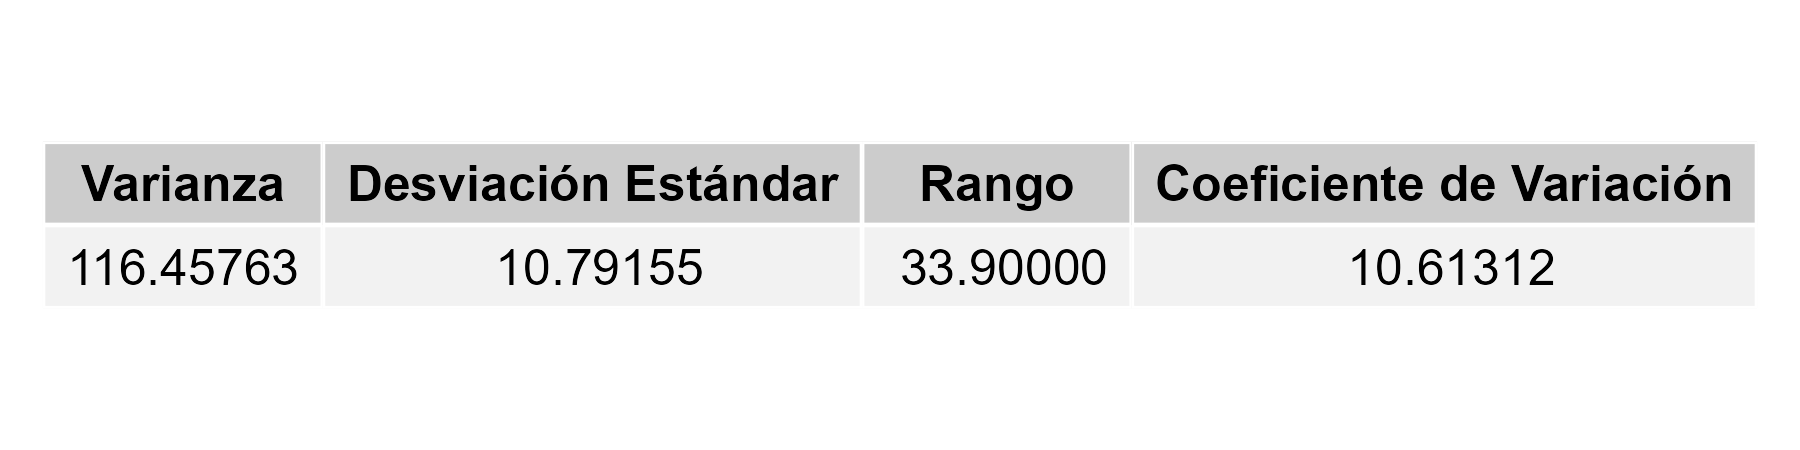
\includegraphics[width=\textwidth]{MTC/GNP.deflator_dispersion.png}
        \caption{Medidas de Dispersión para GNP.deflator}
    \end{figure}
    
    \item \textbf{GNP (Gross National Product)}
    \begin{itemize}
        \item \textbf{Descripción:} Producto Nacional Bruto en millones de dólares.
        \item \textbf{Escala:} Cuantitativa Continua.
        \item \textbf{Significado:} Mide el valor total de los bienes y servicios producidos por la economía de un país, incluyendo los ingresos del extranjero. Indica la salud económica general.
    \end{itemize}
    \begin{figure}[H]
        \centering
        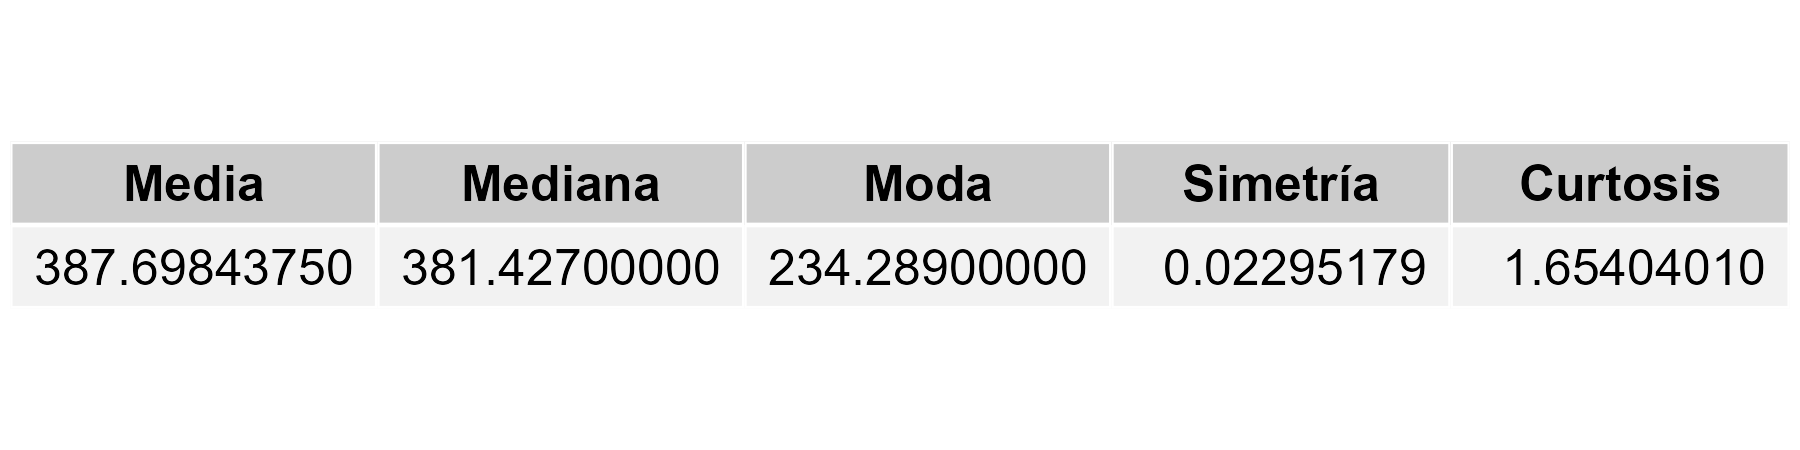
\includegraphics[width=\textwidth]{MTC/GNP_central.png}
        \caption{Medidas de Tendencia Central para GNP}
    \end{figure}
    \begin{figure}[H]
        \centering
        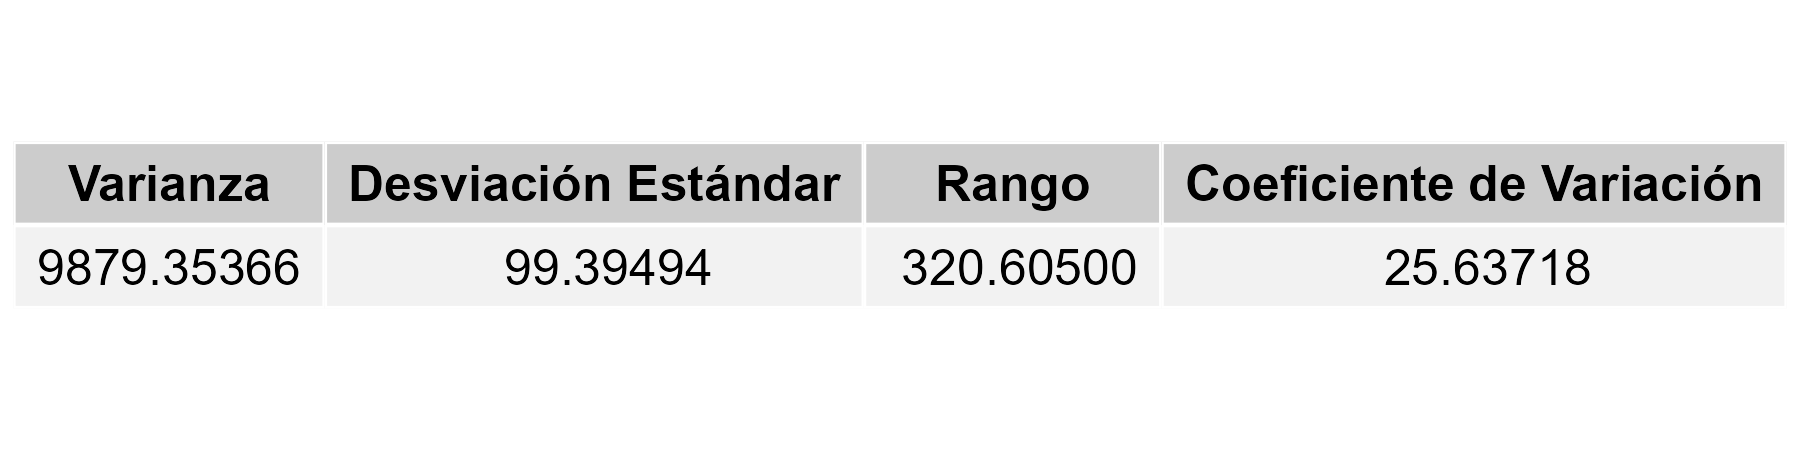
\includegraphics[width=\textwidth]{MTC/GNP_dispersion.png}
        \caption{Medidas de Dispersión para GNP}
    \end{figure}
    
    \item \textbf{Unemployed}
    \begin{itemize}
        \item \textbf{Descripción:} Número de personas desempleadas en miles.
        \item \textbf{Escala:} Cuantitativa Continua.
        \item \textbf{Significado:} Representa la cantidad de personas en la fuerza laboral que están buscando trabajo pero no tienen empleo.
    \end{itemize}
    \begin{figure}[H]
        \centering
        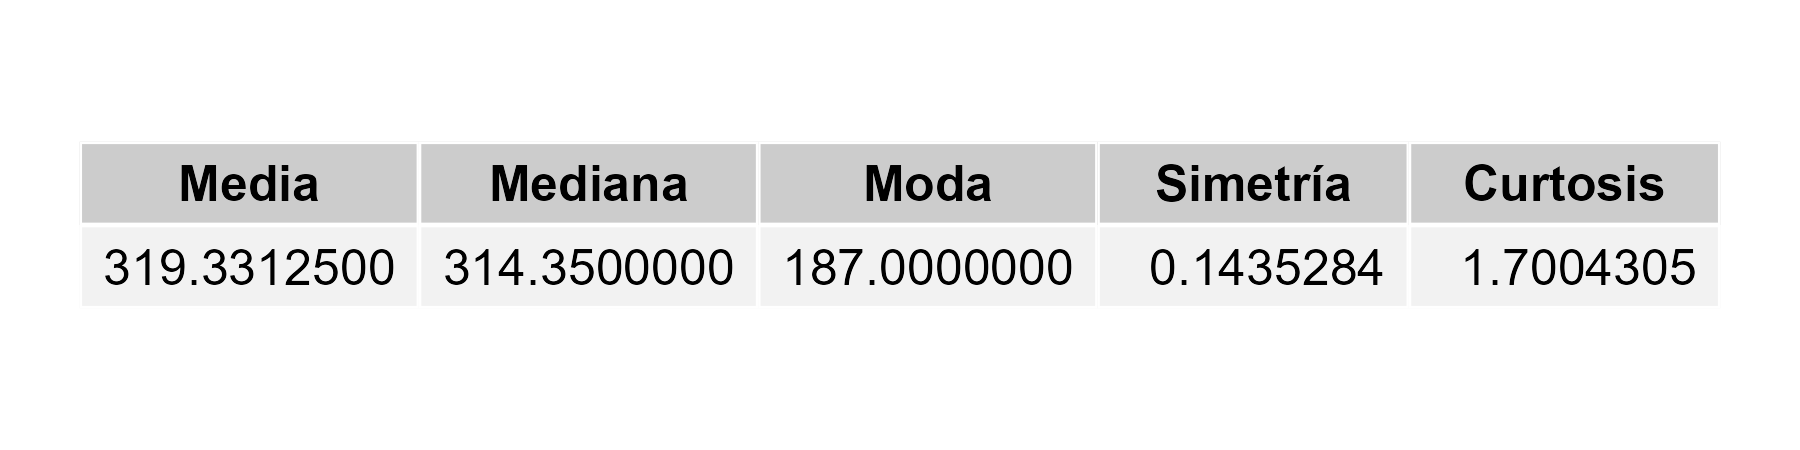
\includegraphics[width=\textwidth]{MTC/Unemployed_central.png}
        \caption{Medidas de Tendencia Central para Unemployed}
    \end{figure}
    \begin{figure}[H]
        \centering
        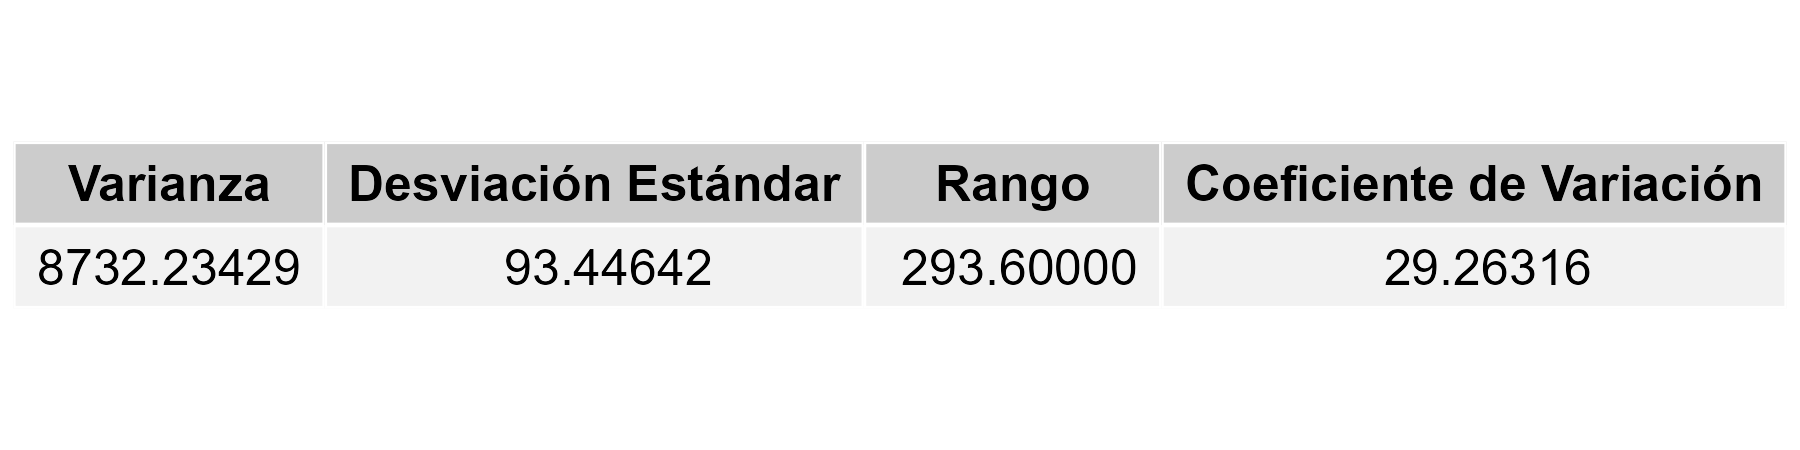
\includegraphics[width=\textwidth]{MTC/Unemployed_dispersion.png}
        \caption{Medidas de Dispersión para Unemployed}
    \end{figure}
    
    \item \textbf{Armed.Forces}
    \begin{itemize}
        \item \textbf{Descripción:} Número de personas enlistadas en las fuerzas armadas en miles.
        \item \textbf{Escala:} Cuantitativa Continua.
        \item \textbf{Significado:} Indica el tamaño de la fuerza laboral militar activa en la economía.
    \end{itemize}
    \begin{figure}[H]
        \centering
        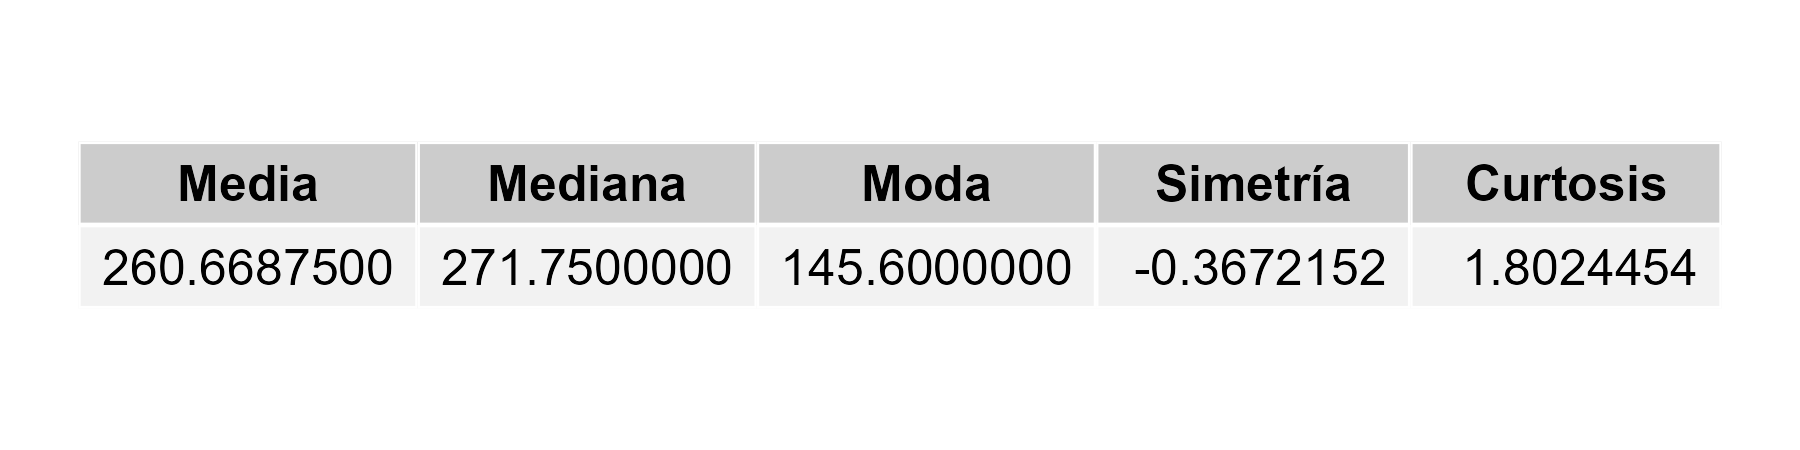
\includegraphics[width=\textwidth]{MTC/Armed.Forces_central.png}
        \caption{Medidas de Tendencia Central para Armed.Forces}
    \end{figure}
    \begin{figure}[H]
        \centering
        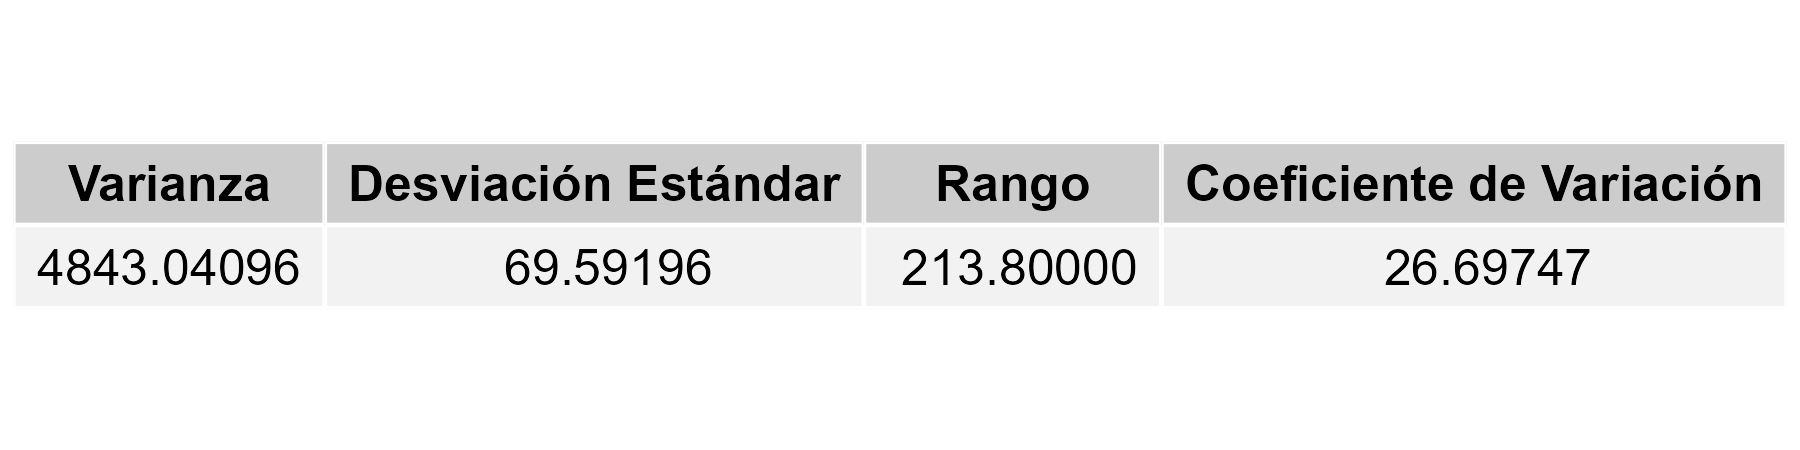
\includegraphics[width=\textwidth]{MTC/Armed.Forces_dispersion.png}
        \caption{Medidas de Dispersión para Armed.Forces}
    \end{figure}
    
    \item \textbf{Population}
    \begin{itemize}
        \item \textbf{Descripción:} Tamaño de la población en miles.
        \item \textbf{Escala:} Cuantitativa Continua.
        \item \textbf{Significado:} Refleja el tamaño total de la población en un determinado año. Es un indicador demográfico que puede influir en variables económicas.
    \end{itemize}
    \begin{figure}[H]
        \centering
        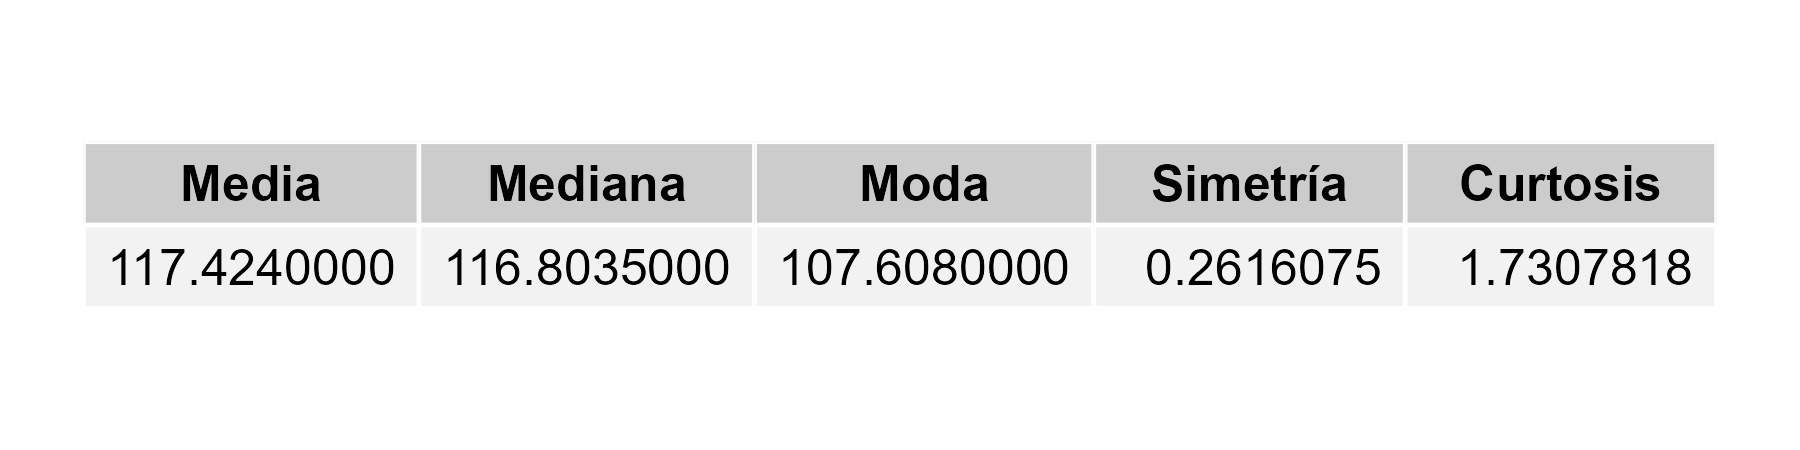
\includegraphics[width=\textwidth]{MTC/Population_central.png}
        \caption{Medidas de Tendencia Central para Population}
    \end{figure}
    \begin{figure}[H]
        \centering
        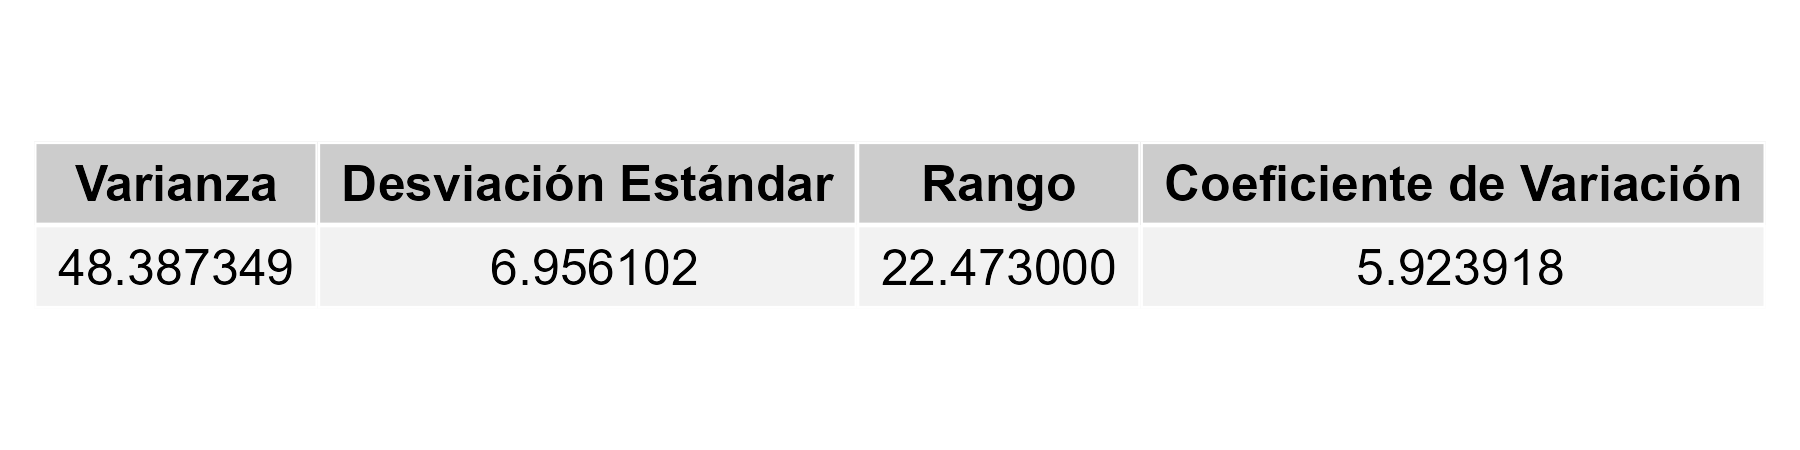
\includegraphics[width=\textwidth]{MTC/Population_dispersion.png}
        \caption{Medidas de Dispersión para Population}
    \end{figure}
    
    \item \textbf{Year}
    \begin{itemize}
        \item \textbf{Descripción:} Año de los datos registrados.
        \item \textbf{Escala:} Cuantitativa Discreta.
        \item \textbf{Significado:} Representa el año específico en el que se registraron los datos.
    \end{itemize}
    \begin{figure}[H]
        \centering
        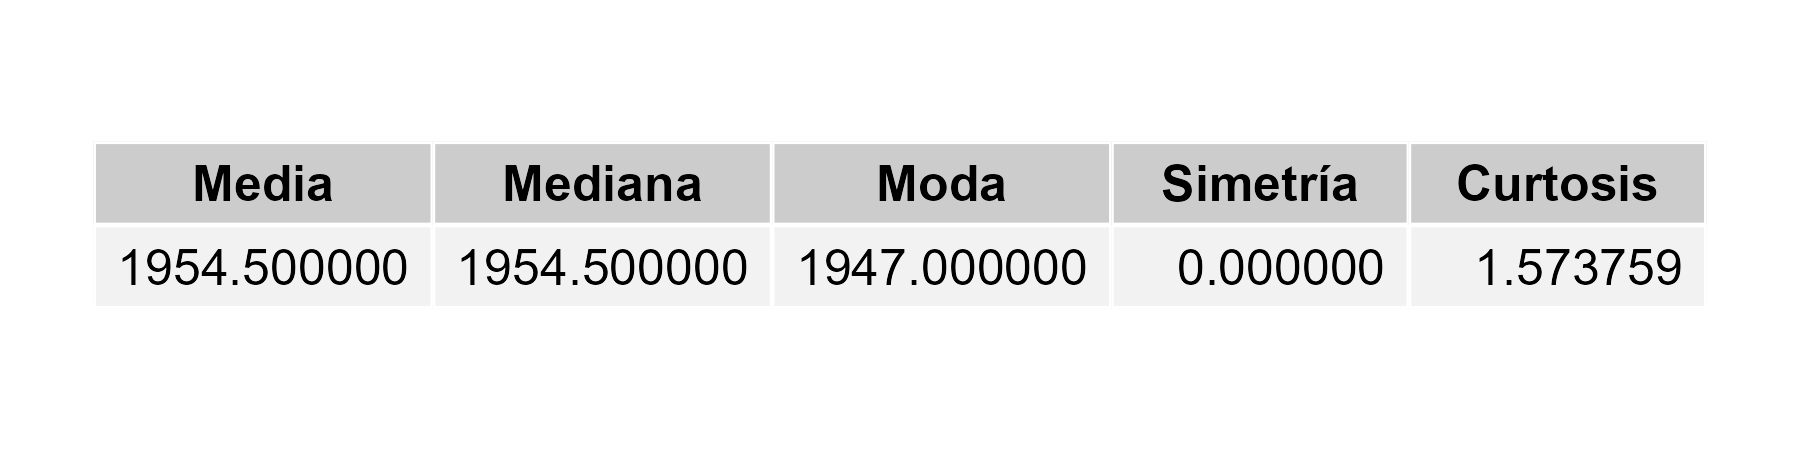
\includegraphics[width=\textwidth]{MTC/Year_central.png}
        \caption{Medidas de Tendencia Central para Year}
    \end{figure}
    \begin{figure}[H]
        \centering
        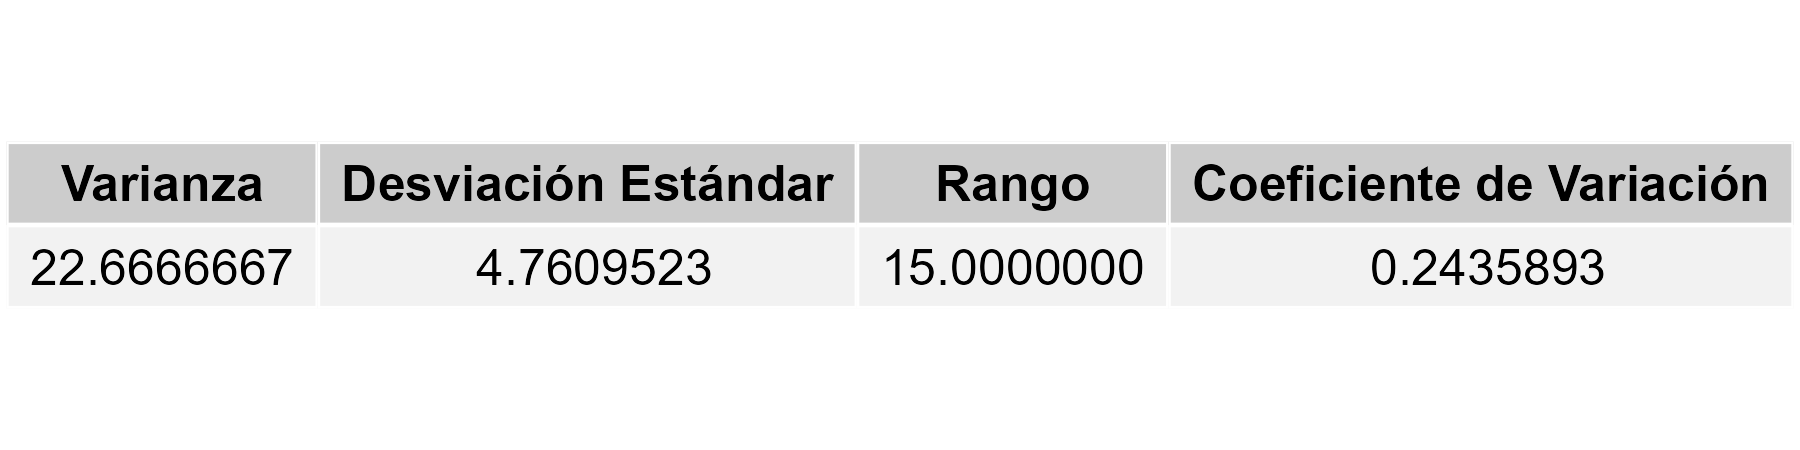
\includegraphics[width=\textwidth]{MTC/Year_dispersion.png}
        \caption{Medidas de Dispersión para Year}
    \end{figure}
    
    \item \textbf{Employed}
    \begin{itemize}
        \item \textbf{Descripción:} Número de personas empleadas en miles.
        \item \textbf{Escala:} Cuantitativa Continua.
        \item \textbf{Significado:} Indica la cantidad de personas que tienen empleo en la economía, lo cual refleja la actividad económica y la salud del mercado laboral.
    \end{itemize}
    \begin{figure}[H]
        \centering
        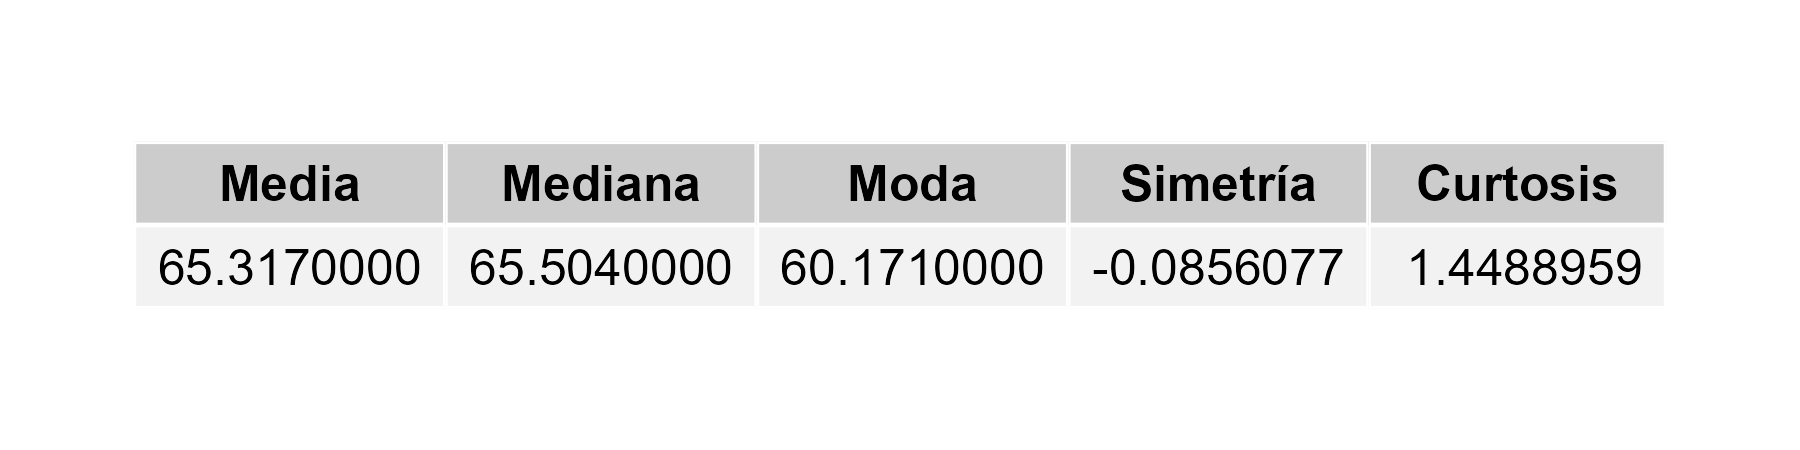
\includegraphics[width=\textwidth]{MTC/Employed_central.png}
        \caption{Medidas de Tendencia Central para Employed}
    \end{figure}
    \begin{figure}[H]
        \centering
        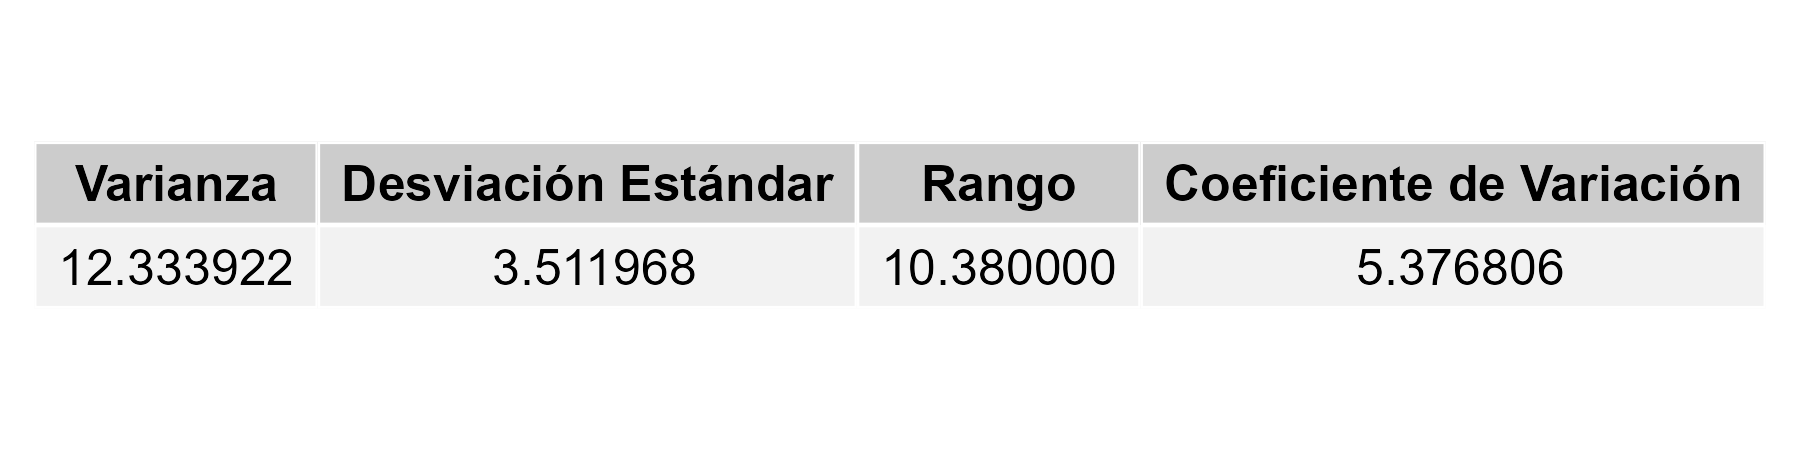
\includegraphics[width=\textwidth]{MTC/Employed_dispersion.png}
        \caption{Medidas de Dispersión para Employed}
    \end{figure}
\end{itemize}




\section{Análisis de la Matriz de Correlación}

\subsection{Correlaciones Fuertes Positivas}

\begin{itemize}
    \item \textbf{GNP.deflator y GNP}: 0.991\\
    Esto indica una relación muy fuerte entre el deflactor del PNB y el PNB en sí. A medida que el PNB aumenta, el deflactor también tiende a aumentar, lo que es esperado en la práctica económica.
    
    \item \textbf{GNP y Employed}: 0.998\\
    Hay una correlación casi perfecta entre el PNB y el número de empleados. Esto sugiere que un aumento en el PNB está fuertemente asociado con un aumento en el empleo.
    
    \item \textbf{Population y Employed}: 0.999\\
    La población y el empleo también están altamente correlacionados. A medida que la población crece, el número de empleados tiende a aumentar, lo que es lógico en un contexto de crecimiento demográfico.
\end{itemize}

\subsection{Correlaciones Fuertes Negativas}

\begin{itemize}
    \item \textbf{Unemployed y GNP}: -0.947\\
    Esta correlación negativa indica que a medida que el PNB aumenta, el número de desempleados tiende a disminuir. Esto es un hallazgo común en la economía, donde un crecimiento económico generalmente se asocia con una disminución del desempleo.
    
    \item \textbf{Unemployed y Employed}: -0.962\\
    Existe una fuerte correlación negativa entre el número de desempleados y el número de empleados. Esto indica que cuando hay más personas empleadas, hay menos desempleados, lo que es un resultado esperado.
\end{itemize}

\subsection{Correlaciones Moderadas}

\begin{itemize}
    \item \textbf{Armed.Forces y Unemployed}: 0.822\\
    Hay una relación positiva moderada entre el número de personas en las fuerzas armadas y el número de desempleados. Esto podría sugerir que en tiempos de conflicto o guerra, más personas se unen a las fuerzas armadas, lo que podría influir en las tasas de desempleo.
    
    \item \textbf{GNP.deflator y Population}: 0.991\\
    La correlación entre el deflactor del PNB y la población es alta, lo que podría indicar que el crecimiento de la población influye en el deflactor.
\end{itemize}

\section{Conclusiones Chi -Cuadrado}

\begin{enumerate}
    \item \textbf{Relaciones Esperadas}: Las correlaciones observadas entre el PNB, el empleo y el desempleo son coherentes con las teorías económicas. Un crecimiento en el PNB generalmente se asocia con un aumento en el empleo y una disminución en el desempleo.
    
    \item \textbf{Colinealidad}: La alta correlación entre variables como GNP, Employed y Population sugiere que hay colinealidad, lo que puede complicar el análisis de regresión. Esto significa que estas variables pueden estar capturando información similar.
    
    \item \textbf{Implicaciones Económicas}: Los hallazgos pueden ser útiles para los formuladores de políticas. Por ejemplo, si se busca reducir el desempleo, se podría considerar estimular el crecimiento del PNB como una estrategia efectiva.
    
    \item \textbf{Limitaciones}: Aunque las correlaciones son informativas, no implican causalidad. Es importante tener en cuenta otros factores que pueden influir en estas relaciones.
\end{enumerate}

\begin{figure}[h] % 'h' indica que la imagen debe aparecer aquí
    \centering % Centra la imagen
    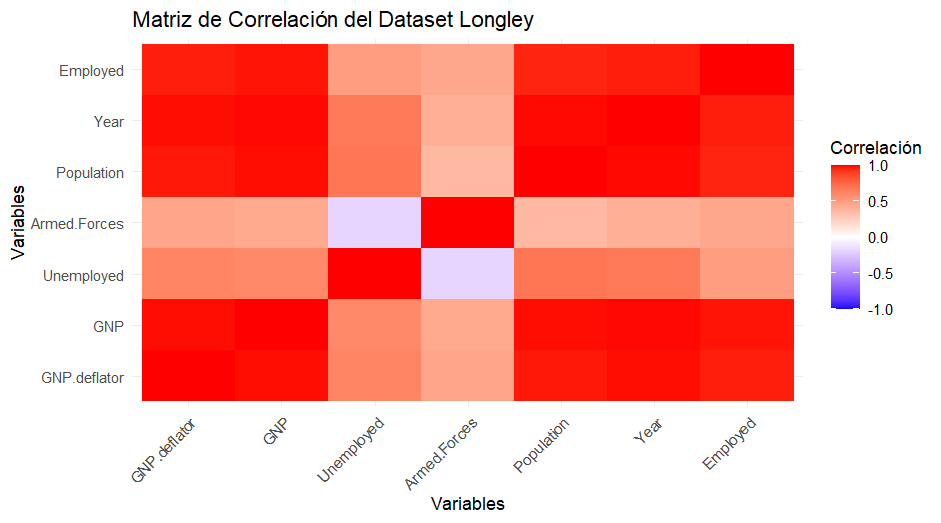
\includegraphics[width=0.8\textwidth]{Correlacion.png}
    \caption{Grafico de Calor , Correlaciones } % Título de la figura
    \label{fig:mi_imagen} % Etiqueta para referencias cruzadas
\end{figure}
\section{Análisis de la Distribucion Normal} Después de ejecutar el código y generar el histograma, podemos observar lo siguiente: \begin{itemize}
    \item El histograma muestra una distribución aproximadamente simétrica y unimodal, lo que indica que los datos siguen una distribución similar a la normal.
    \item La media y la desviación estándar calculadas (representadas por la curva roja) se ajustan bien a la forma del histograma, lo que sugiere que la distribución normal es una buena aproximación para este conjunto de datos.
    \item La mayoría de los valores del Producto Nacional Bruto (GNP) se concentran alrededor de la media, con una disminución gradual hacia los extremos del histograma.
    \item Hay algunos valores atípicos o outliers que se encuentran fuera del rango principal de la distribución, pero en general, los datos se ajustan bien a la curva normal.
    \end{itemize} \section{Interpretación de los Resultados} \begin{itemize}
    \item La distribución normal es una buena aproximación para el Producto Nacional Bruto (GNP) del conjunto de datos Longley, lo que significa que la mayoría de los valores se concentran alrededor de un valor central (la media) y disminuyen simétricamente hacia ambos lados.
    \item La media y la desviación estándar son medidas importantes para describir la distribución normal. La media representa el valor central, mientras que la desviación estándar indica la dispersión de los datos alrededor de la media.
    \item La simetría y unimodalidad del histograma sugieren que no hay evidencia de una distribución bimodal o multimodal, lo que podría indicar la presencia de subgrupos distintos en los datos.
    \item La presencia de algunos valores atípicos puede indicar la existencia de observaciones inusuales o extremas en el conjunto de datos, que podrían requerir un análisis más profundo.
    \end{itemize}
    \begin{figure}[h] % 'h' indica que la imagen debe aparecer aquí
        \centering % Centra la imagen
        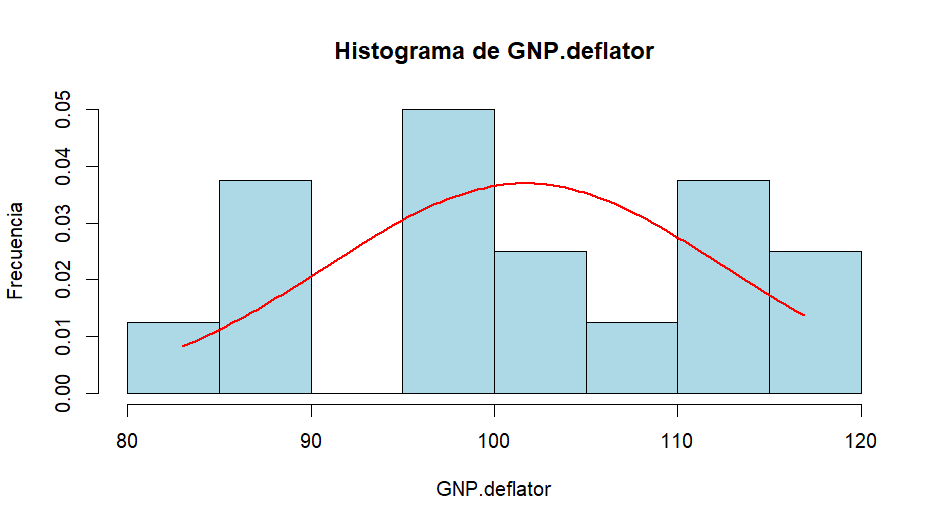
\includegraphics[width=0.8\textwidth]{Normal.png}
        \caption{Distribucion Normal} % Título de la figura
        \label{fig:mi_imagen} % Etiqueta para referencias cruzadas
    \end{figure}
\end{document}
